% !Mode:: "TeX:UTF-8"
\section{\sihao\kai\quad {4.~图片处理}}% 设置目录中章节名、字体、字号及对齐
%%%%%%%%%% 图片处理 %%%%%%%%%%
%%%%%%%%%% 图片处理第一帧 %%%%%%%%%%
\begin{frame}
	\frametitle{\vskip -1.5ex\quad\hei  单个图片及说明}
	\xiaosi \kai
	\begin{figure}% 插入图片
		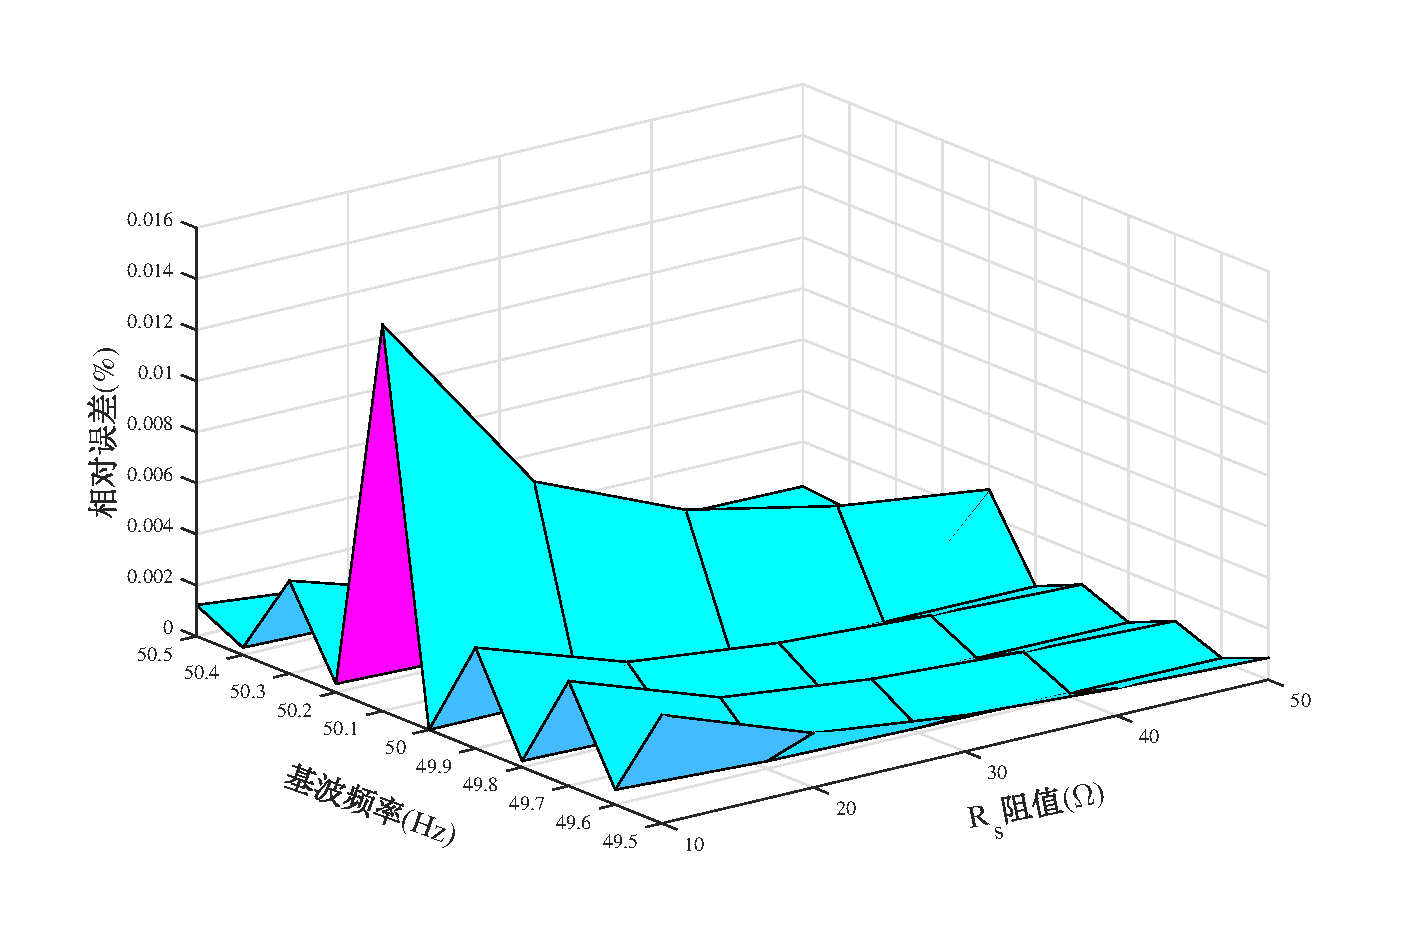
\includegraphics[width=0.9\textwidth]{figures/TR_Fb_TSR}
	\end{figure}
	\vspace{-5.5cm}% 定位说明文字位置,-5.5cm代表从图片下一行处向上移动5.5cm
	% 说明文字(两行)从第2帧之后开始显示,具体位置、字号、字体及高亮显示设置            
	\onslide<2->\qquad\qquad\qquad\qquad \liuhao\kai \alert{当基波频率为~50.1~Hz,$R_s$~为~$10~\Omega$~时误差最大,相对误}\\
	\onslide<2->\qquad\qquad\qquad\qquad\qquad\quad \alert{差不大于~$1.5\times 10^{-2}\%$} \\
	% 定位第二段说明文字位置,为第一段文字后向下移动0.5cm
	\vspace{0.5cm}
	% 说明文字(一行)从第3帧之后开始显示,具体位置、字号、字体及高亮显示设置
	\onslide<3->\qquad\qquad\qquad\qquad\qquad\qquad\qquad \liuhao\kai \alert{随着介损角真值增加,测量误差有逐渐减小的趋势} \\
	% 定位图片标题位置,继续向下移动3.3cm
	\vspace{3.3cm}
	% 图片标题,从第1帧之后开始显示
	\onslide<1->\centering \wuhao 不同阻值条件下的介损角测量误差
\end{frame}
%%%%%%%%%% 图片处理第二帧 %%%%%%%%%%
\begin{frame}
	\frametitle{\vskip -1.5ex\hei\quad 双列图片显示}
	\xiaosi\kai\qquad 窗口长度为~$N=64$~时的~Blackman~窗时频特性
	\begin{figure}
		\centering
		\subfigure[\wuhao 时域特性]{
			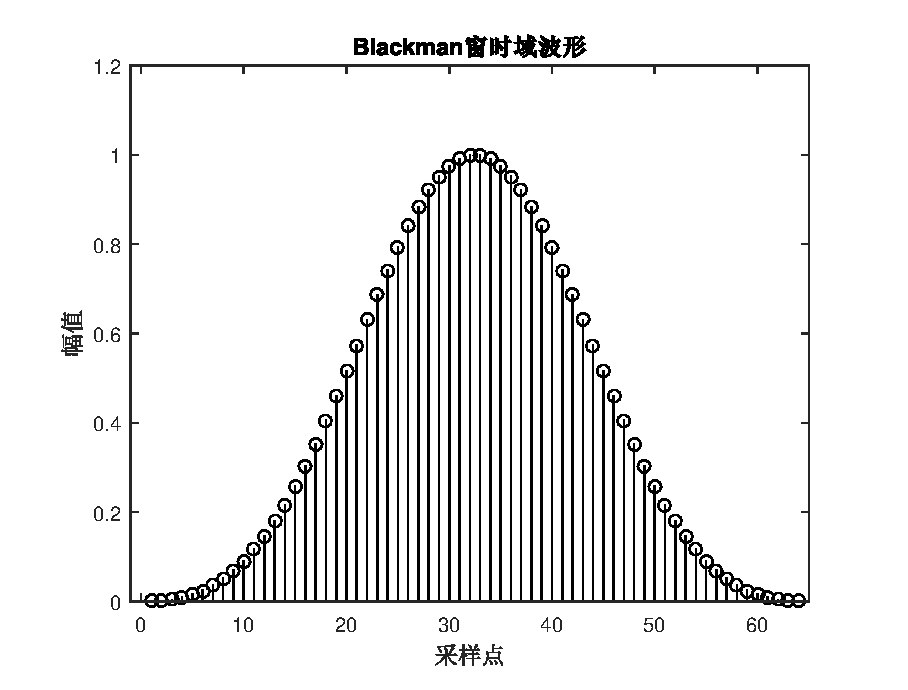
\includegraphics[width=0.45\textwidth]{figures/blackmanTD}}
		\subfigure[\wuhao 幅频特性]{
			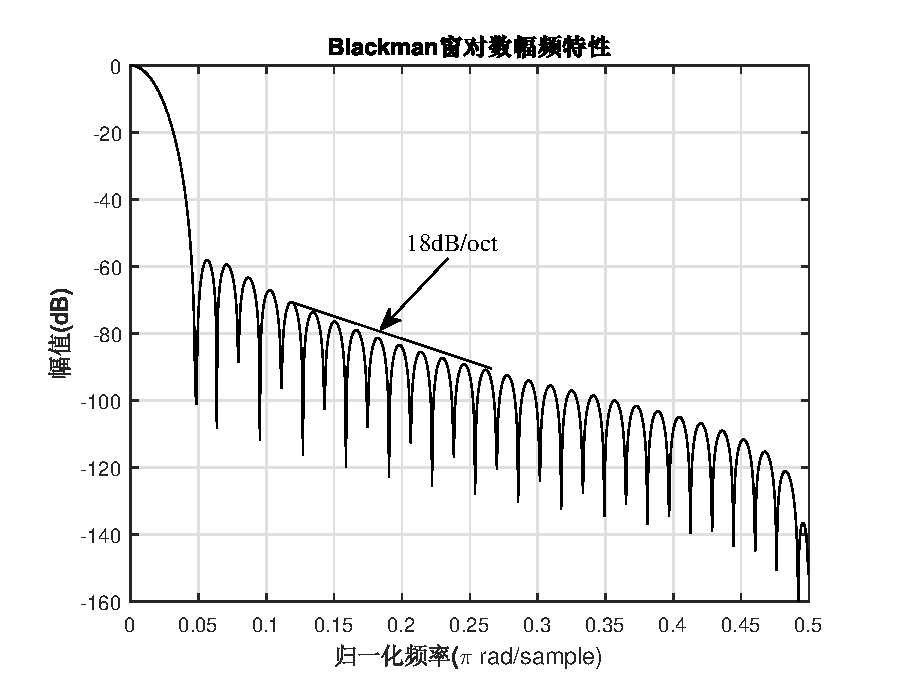
\includegraphics[width=0.45\textwidth]{figures/blackmanAF}}
	\end{figure}
\end{frame}
